%%%%%%%%%%%%%%%%%%%%%%%%%%%%%%%%%%%%%%%%%
% NIWeek 2014 Poster by T. Reveyrand
% www.microwave.fr
% http://www.microwave.fr/LaTeX.html
% ---------------------------------------
%
% Original template created by:
% Brian Amberg (baposter@brian-amberg.de)
%
% This template has been downloaded from:
% http://www.LaTeXTemplates.com
%
% License:
% CC BY-NC-SA 3.0 (http://creativecommons.org/licenses/by-nc-sa/3.0/)
%
%%%%%%%%%%%%%%%%%%%%%%%%%%%%%%%%%%%%%%%%%

%----------------------------------------------------------------------------------------
%	PACKAGES AND OTHER DOCUMENT CONFIGURATIONS
%----------------------------------------------------------------------------------------

\documentclass[a0paper,portrait]{baposter}

\usepackage[T1]{fontenc}
\usepackage{mathtools, graphicx, xurl, hyperref}
% \usepackage{tikz-cd}
\usepackage{tikz}
\usetikzlibrary{shapes, arrows.meta, decorations.pathmorphing, decorations.pathreplacing, backgrounds, positioning, fit, calc, shadows, shapes.misc}
% \tikzexternalize[prefix=tikz/,optimize command away=\includepdf]
\usepackage{boldline, multirow}
\usepackage{booktabs} % Allows the use of \toprule, \midrule and \bottomrule in tables
\usepackage{colortbl}
\usepackage{subcaption}
\usepackage{relsize}
\usepackage{fontawesome5}
\usepackage[ruled, vlined]{algorithm2e}

\usepackage{tabularx} % for 'X' col. type and 'tabularx' environment
\usepackage{ragged2e} % for '\RaggedRight' macro
\newcolumntype{L}{>{\RaggedRight}X} % disable full justification

\usepackage{adjustbox}

% \tikzstyle{smallcircleblock} = [circle, draw, text width = 0.7em, text centered]

% \tikzstyle{wideblock} = [rectangle, draw, text width = 6.5em, text centered, rounded corners, inner sep = 7pt, minimum height = 1.0em]

\newcommand\ImageNode[4][]{
  \node[#1] (#2) {\includegraphics[#3]{#4}};
}
\definecolor{arrowblue}{RGB}{98,145,224}


\newcolumntype{g}{>{\columncolor[gray]{0.8}}l}


\newif\ifcoloredtext
\coloredtextfalse

\newif\ifboxednn
\boxednntrue


% --- unify spacing between floats and text (single-/double-column) ---
\setlength{\textfloatsep}{6pt plus 2pt minus 2pt}   % text <-> single-column floats (table/figure)
\setlength{\intextsep}{6pt plus 2pt minus 2pt}      % inline [h] floats
\setlength{\floatsep}{6pt plus 2pt minus 2pt}       % float <-> float (single-column)

\setlength{\dbltextfloatsep}{6pt plus 2pt minus 2pt} % text <-> double-column floats (figure*)
\setlength{\dblfloatsep}{6pt plus 2pt minus 2pt}     % float <-> float (double-column)

% --- caption spacing for tables only ---
\captionsetup[table]{aboveskip=6pt, belowskip=0pt}


\newenvironment{indentedquote}[1]%
{\list{}{\leftmargin=#1\rightmargin=#1}\item[]}%
{\endlist}


\newcommand\wordcount{\input{|"texcount -inc -sum -0 -utf8 -ch -template={SUM} \currfilepath"}}


\usepackage{textcomp}
\usepackage{eso-pic}
\usepackage{enumitem}
\usepackage{hyperref}
\usepackage{fix-cm}

\setlist[itemize]{
  itemsep=1.5pt,
  topsep=3pt,
  parsep=0pt,
  partopsep=0pt,
  leftmargin=1em,
  labelsep=0.4em
}

\setlength{\abovedisplayskip}{1.5pt plus 1pt minus 1pt}
\setlength{\belowdisplayskip}{1.5pt plus 1pt minus 1pt}

\graphicspath{{images/}} % Directory in which figures are stored

\definecolor{bordercol}{RGB}{40,40,40} % Border color of content boxes
\definecolor{headercol1}{RGB}{186,215,230} % Background color for the header in the content boxes (left side)
\definecolor{headercol2}{RGB}{120,120,120} % Background color for the header in the content boxes (right side)
\definecolor{headerfontcol}{RGB}{0,0,0} % Text color for the header text in the content boxes
\definecolor{boxcolor}{RGB}{210,235,250} % Background color for the content in the content boxes

\definecolor{jdhblue}{RGB}{2,93,186}

\definecolor{zkblue}{RGB}{88,135,175}
\definecolor{zkbackground}{RGB}{230,232,234}


% \usetikzlibrary{shapes, arrows, external, decorations.pathmorphing, backgrounds, positioning, fit, petri, calc, hobby, cd}


\begin{document}

% \background{ % Set the background to an image (background.pdf)
% \begin{tikzpicture}[remember picture,overlay]
% \draw (current page.north west)+(-2em,2em) node[anchor=north west]
% {\includegraphics[height=1.1\textheight]{images/baposter_background.pdf}};
% \end{tikzpicture}
% }

% add conference banner
\AddToShipoutPictureFG*{%
  \AtPageLowerLeft{%
    \hspace{0.77em}
    \raisebox{0.2ex}{
\includegraphics[width=0.147\textwidth]{cinc2025-banner.png}}
  }
}

\begin{poster}{
grid=false,
borderColor=bordercol, % Border color of content boxes
headerColorOne=headercol1, % Background color for the header in the content boxes (left side)
headerColorTwo=headercol2, % Background color for the header in the content boxes (right side)
headerFontColor=headerfontcol, % Text color for the header text in the content boxes
% boxColorOne=boxcolor, % Background color for the content in the content boxes
boxColorOne=zkbackground,
headershape=roundedright, % Specify the rounded corner in the content box headers
headerfont=\Large\sf\bf, % Font modifiers for the text in the content box headers
textborder=rectangle,
% background=user,
background=none,
headerborder=open, % Change to closed for a line under the content box headers
boxshade=plain
}
%
%----------------------------------------------------------------------------------------
%	TITLE AND AUTHOR NAME
%----------------------------------------------------------------------------------------
%
{
\includegraphics[scale=0.385]{logo_cau_science.png}} % University/lab logo
{
{\bf \fontsize{17pt}{17pt} \selectfont Reliability-Aware Hierarchical Learning for Chagas Detection from ECG under Expert Label Scarcity}
} % Poster title
{\vspace{0.3em} \smaller Hao WEN$^1$, Jingsu KANG$^2$  \\  % Author names

$^1${\it College of Science, China Agricultural University}\qquad
$^2${\it Tianjin Medical University} \\
\vspace{0.2cm}
{\Large \bf{The George B. Moody PhysioNet Challenge 2025}, ~~~\bf{Team Revenger}}
}
{
\includegraphics[scale=0.097]{logo_tmu.jpeg}}


\newif\ifcoloredtext
\coloredtexttrue
\newif\ifboxednn
\boxednntrue


%----------------------------------------------------------------------------------------
%	INTRODUCTION & CHALLENGE CONTEXT
%----------------------------------------------------------------------------------------

\headerbox{Framework Summary \& Key Components}{name=introduction, column=0, row=0, span=3}{

\begin{itemize}
\item We propose a \textbf{reliability-aware hierarchical framework} for ECG-based Chagas screening under scarce and noisy labels. The framework comprises three coordinated components: (1) provenance‑stratified label smoothing, (2) moderated source-specific upsampling, and (3) a lightweight variable‑length bottleneck ResNet classifier.
\item The supervision design assigns sharp targets to expert‑confirmed positives, softened targets to self‑reported samples, and mild smoothing to non‑endemic negatives, while distinct upsampling factors amplify scarce reliable positives without collapsing cohort diversity.
\item The encoder stacks 4 bottleneck residual blocks with a global squeeze‑and‑excitation module and global max pooling to handle variable-length inputs; training couples reliability‑coded targets with an asymmetric loss to concentrate learning on hard positives amid severe class imbalance.
\end{itemize}
}

%----------------------------------------------------------------------------------------
%	DATA
%----------------------------------------------------------------------------------------

\headerbox{Dataset Preparation}{name=data, column=0, row=1, span=1, below=introduction}{

\begin{itemize}
\item \textbf{Sampling}: All 12-lead ECGs uniformly resampled to 400 Hz.
\item \textbf{Filtering}: Butterworth bandpass 0.5–45 Hz to suppress baseline wander + high-frequency noise.
\item \textbf{Normalization}: Per-record z-score
\begingroup
\setlength{\abovedisplayskip}{2pt}  % 上间距
\setlength{\belowdisplayskip}{2pt}  % 下间距
\[
\tilde{\mathbf{x}} = \frac{\mathbf{x} - \boldsymbol{\mu}_{\mathbf{x}}}{\boldsymbol{\sigma}_{\mathbf{x}}}
\]
\endgroup
to zero mean, unit variance.
\item \textbf{Exclusion criteria}: Discard recordings $<1{,}200$ samples ($<3$ s @ 400 Hz) to ensure enough cardiac cycles.
\end{itemize}

}

%----------------------------------------------------------------------------------------
%	RELIABILITY-AWARE SUPERVISION
%----------------------------------------------------------------------------------------

\headerbox{Reliability-Aware Supervision}{name=supervision, column=1, row=1, span=2, below=introduction}{

% Three ECG datasets with heterogeneous label reliability and Chagas prevalence:

Hierarchical supervision: source reliability levels (expert > self-report > non-endemic negatives) $\longrightarrow$ calibrated label smoothing ($\varepsilon$) + moderated upsampling.

\vspace{-1ex}
% {\smaller[1]
\begin{center}
\begin{tabular}{rlllllll}
\toprule
\multirow{2}{*}{Dataset} & \multirow{2}{*}{Size} & \multirow{2}{*}{Chagas \%} & \multirow{2}{*}{Provenance} & \multirow{2}{*}{Up $\times$} & \multirow{2}{*}{$\varepsilon$} & \multicolumn{2}{c}{Smoothed Targets} \\ \cmidrule(lr){7-8}
& & & & & & negative & positive \\
\midrule
SaMi-Trop   & 1,631     & 100 \%    & expert-confirmed  & $\times$ 12 & 0.0 & N/A           & $[0,\,1]$     \\
CODE-15\%   & 345,779   & 1.795 \%  & self-reported     & $\times$ 3  & 0.6 & $[0.7,\,0.3]$ & $[0.3,\,0.7]$ \\
PTB-XL      & 21,799    & 0 \%      & non-endemic (neg) & $\times$ 1  & 0.2 & $[0.9,\,0.1]$ & N/A           \\
\bottomrule
\end{tabular}
\end{center}
% }
\vspace{-1ex}

Label smoothing (binary, $C=2$): $\tilde{\mathbf{y}} = (1 - \varepsilon) \cdot {\mathbf{y}} + \frac{\varepsilon}{C} \cdot {\mathbf{1}}$.

\begin{itemize}
% \item Reliability levels: expert (sharp, high upsampling) > self-report (soft, moderate) > non-endemic negatives (mild).
\item Purpose: reduce overconfident gradients for noisier self-reports while preserving expert signal.
% \item Upsampling balance: (CODE-15\% $\times$3, SaMi-Trop $\times$12) maximized hidden score; aggressive (10,120) overfit / degraded generalization.
% \item PTB-XL adds negative morphology diversity; mild smoothing (0.2) regularizes the decision boundary.
% \item Interaction: provenance-aware smoothing complements asymmetric loss (ASL) by encoding prior trust.
\item Benefit: replaces ad-hoc class weights with structured priors; stabilizes early training variance.
% \item Limitation: $\varepsilon$ values are manually fixed—do not capture intra-source heterogeneity (future: learn instance reliability).
\item Complementarity: provenance-based smoothing reduces label noise impact; ASL (asymmetric loss) focuses capacity on hard positives:
\begingroup
\setlength{\abovedisplayskip}{2pt}  % 上间距
\setlength{\belowdisplayskip}{2pt}  % 下间距
\[
\operatorname{ASL} = -y \cdot (1-p)^{\gamma_{+}} \log(p) - (1-y) \cdot (p_m)^{\gamma_{-}} \log(1-p_m)
\]
\endgroup
where $p$ is the predicted probability of the positive class, $y$ is the (smoothed) positive-class target probability, $p_m = \max(p - m, 0),$ $(\gamma_{+},\gamma_{-})=(1,4)$ and margin $m=0.05$.
\end{itemize}

}

%----------------------------------------------------------------------------------------
%	MODEL ARCHITECTURE
%----------------------------------------------------------------------------------------

\headerbox{Model Architecture}{name=model, column=0, row=2, span=1, below=data}{

{\bf Enhanced 1D ResNet with SE Modules}

\vspace{-2.5ex}

\begin{center}
\resizebox{1.03\linewidth}{!}{%
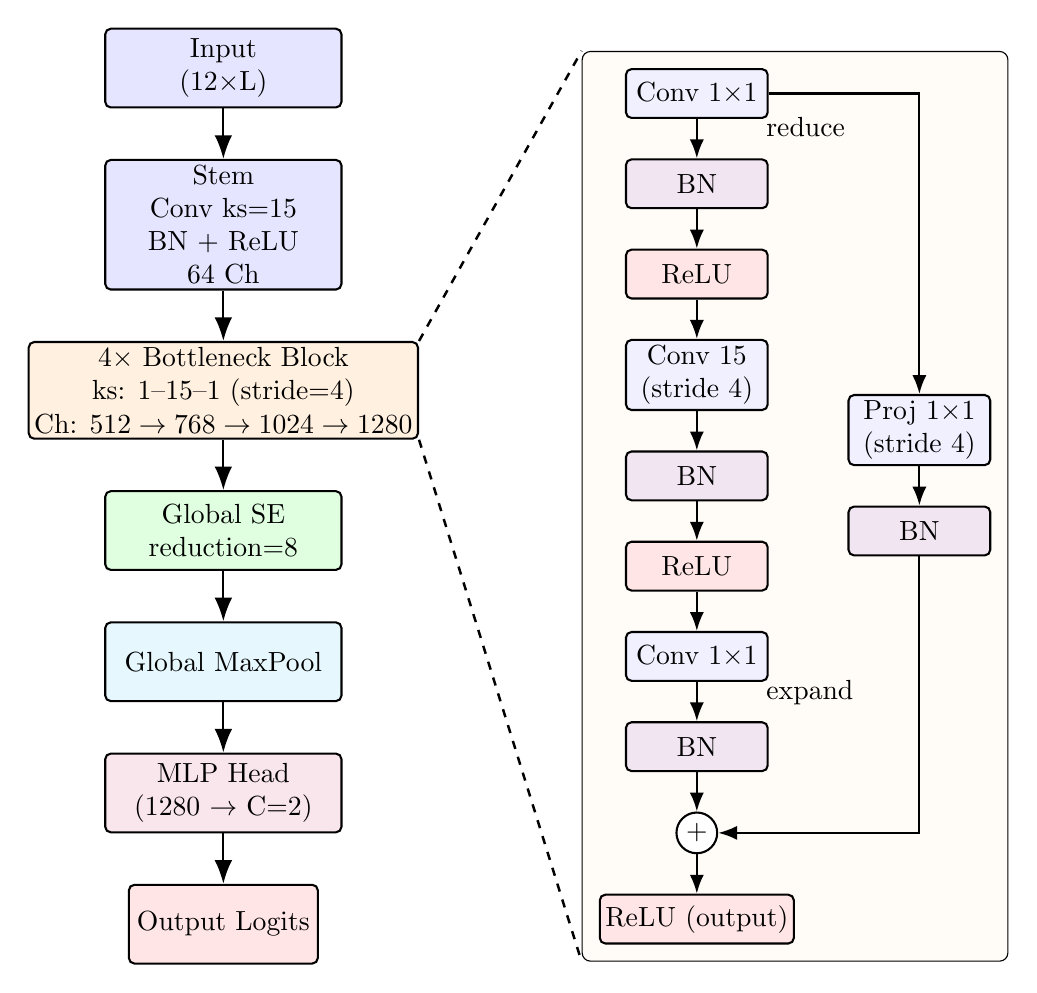
\begin{tikzpicture}[
    % font=\small,
    line width=0.75pt,
    >={Latex[length=3mm]},
    node distance=6.4mm,
    every node/.style={inner sep=2pt},
    stem/.style={draw, rounded corners=2pt, minimum width=30mm, minimum height=10mm,
                 align=center, fill=blue!10},
    block/.style={draw, rounded corners=2pt, minimum width=30mm, minimum height=12mm,
                  align=center, fill=orange!12},
    se/.style={draw, rounded corners=2pt, minimum width=30mm, minimum height=10mm,
               align=center, fill=green!12},
    pool/.style={draw, rounded corners=2pt, minimum width=30mm, minimum height=10mm,
                 align=center, fill=cyan!10},
    head/.style={draw, rounded corners=2pt, minimum width=30mm, minimum height=10mm,
                 align=center, fill=purple!10},
    output/.style={draw, rounded corners=2pt, minimum width=24mm, minimum height=10mm,
                align=center, fill=red!10},
    arrow/.style={-{Latex[length=3mm]}, thick},
    darr/.style={-{Latex[length=2.4mm]}, thick},
    dashedarrow/.style={-{Latex[length=2.6mm]}, thick, dashed},
    ann/.style={inner sep=1pt, align=center},
    layer/.style={draw, rounded corners=2pt, minimum width=18mm, minimum height=6.2mm,
                  align=center, fill=blue!6},
    bnact/.style={draw, rounded corners=2pt, minimum width=18mm, minimum height=6.2mm,
                  align=center, fill=violet!10},
    act/.style={draw, rounded corners=2pt, minimum width=18mm, minimum height=6.2mm,
                  align=center, fill=red!10},
    drop/.style={draw, rounded corners=2pt, minimum width=18mm, minimum height=6.2mm,
                  align=center, fill=gray!15, dashed},
    sum/.style={draw, circle, inner sep=1.6pt, fill=white},
    % brace/.style={decorate, decoration={brace, amplitude=6pt}},
    detailbox/.style={draw, rounded corners=3pt, inner sep=6pt, fill=orange!3}
]

% ================= Left (overall vertical path) =================
\node[stem] (input) {Input \\ (12$\times$L)};
\node[stem, below=of input] (stem) {Stem \\ Conv ks=15 \\ BN + ReLU \\ 64 Ch};

% Compressed single bottleneck block (represents 4 stacked blocks)
\node[block, below=of stem] (bottleneck) {$4 \times$ Bottleneck Block \\ ks: 1--15--1 (stride=4) \\ Ch: $512 \to 768 \to 1024 \to 1280$};

% Global SE
\node[se, below=of bottleneck] (gse) {Global SE \\ reduction=8};

% Global pooling
\node[pool, below=of gse] (gap) {Global MaxPool};

% MLP Head
\node[head, below=of gap] (mlp) {MLP Head \\ (1280 $\rightarrow$ C=2)};

% Output
\node[output, below=of mlp] (out) {Output Logits};

% Arrows (overall path)
\draw[arrow] (input) -- (stem);
\draw[arrow] (stem) -- (bottleneck);
\draw[arrow] (bottleneck) -- (gse);
\draw[arrow] (gse) -- (gap);
\draw[arrow] (gap) -- (mlp);
\draw[arrow] (mlp) -- (out);

% ================= Right (expanded single bottleneck internals) =================
% Anchor for expansion (to the right of overall bottleneck block)
\coordinate (expandAnchor) at ($(input.east)+(45mm,0)$);

\node[layer, below=0mm of expandAnchor] (c1) {Conv 1$\times$1};
\node[below right=-1mm and 8mm of c1.south] {reduce};
\node[bnact, below=5mm of c1] (bn1) {BN};
\node[act, below=5mm of bn1] (a1) {ReLU};

\node[layer, below=5mm of a1] (c2) {Conv 15\\(stride 4)};
\node[bnact, below=5mm of c2] (bn2) {BN};
\node[act, below=5mm of bn2] (a2) {ReLU};
% \node[drop, below=5mm of a2] (drp) {Dropout 0.2};

\node[layer, below=5mm of a2] (c3) {Conv 1$\times$1};
\node[below right=-1mm and 8mm of c3.south] {expand};
\node[bnact, below=5mm of c3] (bn3) {BN};

\node[sum, below=5mm of bn3] (add) {+};
\node[act, below=5mm of add] (outact) {ReLU (output)};

% Projection/skip branch (since stride=4 or channel change)
\node[layer, right=10mm of c2, yshift=-7mm, minimum width=18mm] (proj) {Proj 1$\times$1 \\ (stride 4)};
\node[bnact, below=5mm of proj, minimum width=18mm] (projbn) {BN};

% Connections internal
\draw[darr] (c1) -- (bn1);
\draw[darr] (bn1) -- (a1);
\draw[darr] (a1) -- (c2);
\draw[darr] (c2) -- (bn2);
\draw[darr] (bn2) -- (a2);
% \draw[darr] (a2) -- (drp);
\draw[darr] (a2) -- (c3);
\draw[darr] (c3) -- (bn3);
\draw[darr] (bn3) -- (add);
\draw[darr] (add) -- (outact);

% Skip path
\draw[darr] (c1.east) -| ($(proj.north)+(0,0mm)$);
\draw[darr] (proj) -- (projbn);
\draw[darr] (projbn.south) |- (add.east);

\begin{scope}[on background layer]
\node[detailbox, fit=(c1) (bn1) (a1) (c2) (bn2) (a2) (c3) (bn3) (proj) (projbn) (add) (outact)] (detail) {};
\end{scope}

\draw[dashed, line width=0.9pt] (bottleneck.north east) -- (detail.north west);
\draw[dashed, line width=0.9pt] (bottleneck.south east) -- (detail.south west);

\end{tikzpicture}

}
\end{center}

\vspace{-0.5ex}

\begin{itemize}
\item {\bf Stem}: Conv1d (kernel 15, stride 1, 64 output channels) followed by BN and ReLU, providing initial local morphology modeling.
\item {\bf Bottleneck blocks}: 1-15-1 convolutions, expansion factor 4, stride 4 downsampling
\item {\bf Global SE}: Channel attention, reduction ratio 8 for temporal feature recalibration.
\item {\bf Variable-length inputs}: Global MaxPool enables inference on ECGs of any duration.
% \item {\bf Classification MLP head}: Hidden FC layer ($1280 \to 1024$) with non-linear activation and dropout (rate 0.2), followed by a final linear layer ($1024 \to 2$) producing class logits.
\end{itemize}

}

%----------------------------------------------------------------------------------------
%	UPSAMPLING STRATEGY SELECTION
%----------------------------------------------------------------------------------------

\headerbox{Upsample Strategy Selection}{name=upsampling, column=1, row=2, span=1, below=supervision}{
\small
% \textbf{Goal:} Amplify scarce reliable positives without collapsing inter‑cohort diversity.

\begin{center}
\begin{tabular}{ccc}
\toprule
\multicolumn{2}{c}{Upsample factor} & \multirow{2}{*}{Challenge score} \\ \cmidrule(lr){1-2}
CODE-15\% & SaMi-Trop               &                                  \\ \midrule
-         & -                       & 0.239$^\dagger$                        \\
3         & 7                       & 0.212                            \\
3         & 12                      & \textbf{0.245}                   \\
10        & 120                     & 0.210                            \\
6         & 36                      & 0.221                            \\
\bottomrule
\end{tabular}
\end{center}
\vspace{-1ex}
$^\dagger$ obtained during the unofficial phase.

\begin{itemize}
\item Moderate replication outperformed both no upsampling and extreme factors.
\item Extreme factors increased memorization and reduced hidden generalization.
% \item PTB-XL (negatives only) kept at ×1 to avoid further skew toward the negative class.
\end{itemize}

}

%----------------------------------------------------------------------------------------
%	TRAINING CONFIGURATION
%----------------------------------------------------------------------------------------

\headerbox{Training Configuration}{name=training, column=2, row=2, span=1, below=supervision}{

\begin{itemize}[leftmargin=8pt,itemsep=2pt,topsep=2pt]
\item \textbf{Optimizer \& scheduler}: AdamW (weight decay $1\times 10^{-2}$) with OneCycle LR over 30 epochs: base $1\times10^{-4} \rightarrow$ peak $6\times10^{-4}$ (early phase) $\rightarrow$ anneal to $\approx 1\times10^{-6}$.
% \item \textbf{Batch / epochs / early stop}: Batch size 128; max 30 epochs; early stopping (patience 10) on a fixed 20\% hold-out subset using the Challenge metric.
\item \textbf{Batch size}: 128.
\item \textbf{Epochs}: Max 30 epochs.
\item \textbf{Early stop}: Patience 10 epochs, evaluated on a fixed 20\% hold-out subset using the Challenge metric.
\item \textbf{Training segments}: Uniform random crop (or center padding if shorter) of 4{,}096 samples.
\item \textbf{Implementation}: PyTorch + \texttt{torch-ECG} framework

\end{itemize}
}

%----------------------------------------------------------------------------------------
%	RESULTS
%----------------------------------------------------------------------------------------

\headerbox{Results}{name=results, column=1, row=3, span=2, below=upsampling}{

% {\bf Challenge Performance \& Analysis}

\begin{center}
\begin{tabular}{r|r|r|r}
Internal hold-out (mean±std) & Hidden validation & Test & Ranking \\
\hline
$0.451 \pm 0.005$ & 0.245 & 0.163 & 32~/~40 \\
\hline
\end{tabular}
\end{center}
\vspace{-1ex}
The rankings are based on the hidden test set. Results on the public training data (more specifically, the hold-out subset) are also provided for reference.

}

%----------------------------------------------------------------------------------------
%	DISCUSSION & Limitations
%----------------------------------------------------------------------------------------

\headerbox{Discussion \& Limitations}{name=discussion, column=0, row=4, span=3, below=results}{

\begin{itemize}
\item Our reliability-aware hierarchical framework provides a lightweight, supervision-centric route to Chagas ECG screening under scarce positives and mixed label noise, without relying on heavy architectures or pretraining.
\item The generalization gap (internal hold-out vs hidden validation) suggests residual distribution shift (cohort composition/prevalence) and under-adaptation of our fixed supervision scheme.
\item Static supervision limits adaptation: (i) Fixed smoothing factors ($\varepsilon$) capture only coarse provenance, missing intra-source label quality variation; (ii) dataset-level upsampling with fixed multipliers ignores evolving model confidence and per-instance difficulty.
\item \textbf{Future directions}:
\begin{itemize}
\item Adaptive supervision: jointly learn instance-level reliability weights and adjust positive sampling (curriculum/difficulty- or confidence-aware, hard positive mining, etc.) instead of fixed smoothing factors $\varepsilon$ and static upsampling multipliers.
\item Augmentation \& synthesis: CutMix, mixup variants, temporal warping, and class-conditional synthesis to expand minority morphology diversity.
\item Multi-task \& pretraining: leverage arrhythmia / morphology labels; self-supervised ECG representation learning before supervised fine-tuning.
\end{itemize}
\end{itemize}

}

%----------------------------------------------------------------------------------------
%	FOOTER
%----------------------------------------------------------------------------------------

\headerbox{}{name=foottext, column=0, span=3, below=discussion, textborder=none, headerborder=none, boxheaderheight=0pt}{
\hfill \small \textit{Code, configs, etc. are available at https://github.com/wenh06/cinc2025, and is based on https://github.com/DeepPSP/torch\_ecg.}
}

\end{poster}

\end{document}
